% ----------------------------------------

\subsection{Environment behavior}

% ----------------------------------------

\begin{frame}
\frametitle{Non-stationary behavior}
\framesubtitle{Overview}

By using the \textbf{non-stationarity} assumption we are taking into consideration that the demand curve could be subject to changes over time and isn't necessarily fixed as we have seen in other steps.

There are 2 main types of \textit{non-stationary behaviors}:
\begin{itemize}[label={$\circ$}]
    \item \textbf{Abrupt changes}: where it's possible to identify different phases with different phase-wise stationary demand curves.
    \item \textbf{Smooth changes}: where the demand curve changes over time in a continuous manner.
\end{itemize}

As per specifications, we will only consider \textbf{abrupt changes} in the scope of our project.

\end{frame}

% ----------------------------------------

\begin{frame}
\frametitle{Non-stationary behavior}
\framesubtitle{Abrupt changes}

\textbf{Abrupt changes} are usually experienced when an important event strikes the market \textit{(e.g. a new product that shifts the interests of the users is released or an historical event shapes the opionion of people)}; change isn't necessarily bad, however, it may impact negatively the prediction of learners that were created with a static environment in mind.

Neither \textbf{UCB} nor \textbf{TS} account for abrupt changes since it's almost impossible for them to try a superarm that was deemed as \textit{unoptimal} over the past iterations (while it might have become optimal after an \textit{abrupt change}), therefore we expect to see a significant \textbf{reward drop} from them after an \textit{abrupt change}.

\end{frame}

% ----------------------------------------

\begin{frame}
\frametitle{Simulating abrupt changes}

In the early stages of the project we noticed that the \textbf{Simulation} that we created wasn't really fit to dinamically include abrupt changes in the environment, therefore great effort was spent in completely reworking the interface for the \textbf{Simulation} from the ground-up.

Besides collateral improvements in reproducibility, results collection and user-friendliness, the new \textbf{Simulation} allowed for an \textit{incremental simulation unfolding}, this meant that we were now able to simulate \textit{n} days, change the environment and simulate another \textit{n} days.

This particular feature revealed itself as fundamental for the upcoming challenges.

\end{frame}

% ----------------------------------------

\subsection{Algorithms}

% ----------------------------------------

\begin{frame}
\frametitle{Approaches}
\framesubtitle{Sliding window and Change detection}

There are 2 main approaches to deal with a \textbf{non-stationary environment}
\begin{itemize}[label={$\circ$}]
    \item \textbf{Sliding window}: only consider the last $\tau$ samples for predictions.
    \item \textbf{Change detection}: detect when a change has happened and adapt accordingly.
\end{itemize}

It's clear that \textbf{Sliding window} approaches are more fit for \textbf{smooth changes} while \textbf{Change detection} approaches work better with \textbf{abrupt changes}, however it's important to note that both approaches can be utilized to deal with any \textit{non-stationary} scenario.

\end{frame}

% ----------------------------------------

\begin{frame}
\frametitle{Sliding window}
\framesubtitle{Sliding window for TS and UCB}

\begin{itemize}[leftmargin=*, label={$\circ$}]
    \item \textbf{SW-UCB} differs in the confidence bound formulation and the new arm choice:
        \begin{displaymath}
            a_t =
            \begin{cases}
                a_{\overline{t}} & \text{if} ~ \exists \overline{t} \vert n_{a_{\overline{t}}}(t-1, \tau) = 0 \\
                arg\max\limits_{a \in A} \left\{ \overline{x}_{a, t, \tau} + \sqrt{\frac{2log(t)}{n_a(t-1, \tau)}} \right\} & \text{otherwise}
            \end{cases}
        \end{displaymath}
    \item \textbf{SW-TS} differs in the $\beta$ distribution update:
        \begin{displaymath}
            \displayindent0pt \displaywidth\textwidth
            (\alpha_{a_t}, \beta_{a_t}) =
            \begin{cases}
                (\alpha_{a_t}, \beta_{a_t}) + (x_{a_t, t}, 1-x_{a_t, t}) & \text{if} ~ t \leq \tau \\[1ex]
                \!\begin{aligned}
                    & \max \{ (1, 1)\!\begin{aligned}[t]
                        & , (\alpha_{a_t}, \beta_{a_t}) + (x_{a_t, t}, 1-x_{a_t, t}) \\
                        & - (x_{a_{t-\tau}, t-\tau}, 1-x_{a_{t-\tau}, t-\tau}) \}
                    \!\end{aligned}
                \end{aligned} & \text{if} ~ t > \tau
            \end{cases}
        \end{displaymath}
\end{itemize}

\end{frame}

% ----------------------------------------

\begin{frame}
\frametitle{Change detection}

We used a \textbf{reward-based algorithm} as a \textit{change detection algorithm}, it works by comparing the last $k$ rewards with the newest $k$ rewards ($k=4$ by default) and if the difference between their means exceedes a certain threshold $\omega$ ($\omega=400$ by default) the learner is \textbf{reset} and is therefore able to learn a new optimal superarm from scratch.

Formally:
\begin{displaymath}
    \text{RESET learner if} ~ t \geq 2k ~ \land \sum_{i=t-2k}^{t-k} r_i -\sum_{i=t-k+1}^t r_i > \omega
\end{displaymath}

\scriptsize N.B. there is an offset of 1 in the representation of t between theory and code

\end{frame}

% ----------------------------------------

\subsection{Results}

% ----------------------------------------

\begin{frame}
\frametitle{}
\framesubtitle{}

\todo{insert correct image}
%\makebox[\textwidth]{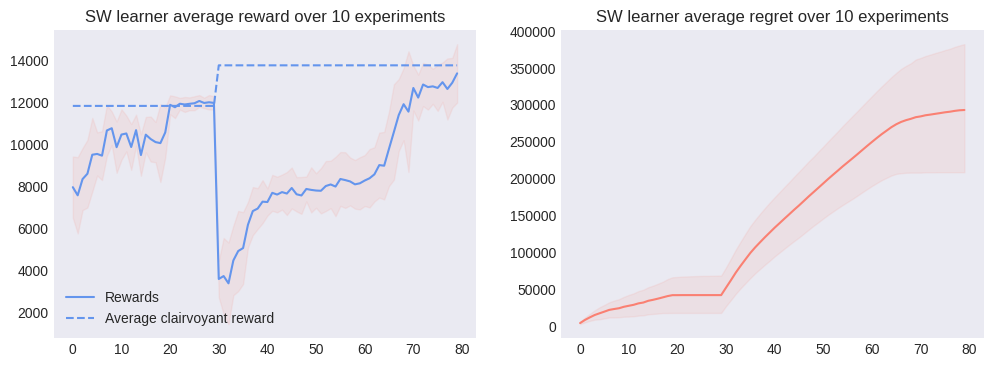
\includegraphics[width=\paperwidth]{img/Graphs/non_stationary/image2.png}}

\scriptsize Graphs representing reward and regret in the non-stationary environment with different approaches. (Only \textbf{UCB} algorithms were evaluated)

\end{frame}

% ----------------------------------------

\begin{frame}
\frametitle{Reward and regret}

We calculated the mean \textbf{reward} and \textbf{regret} considering their variance over multiple runs.

\todo{insert image}
%\makebox[\textwidth]{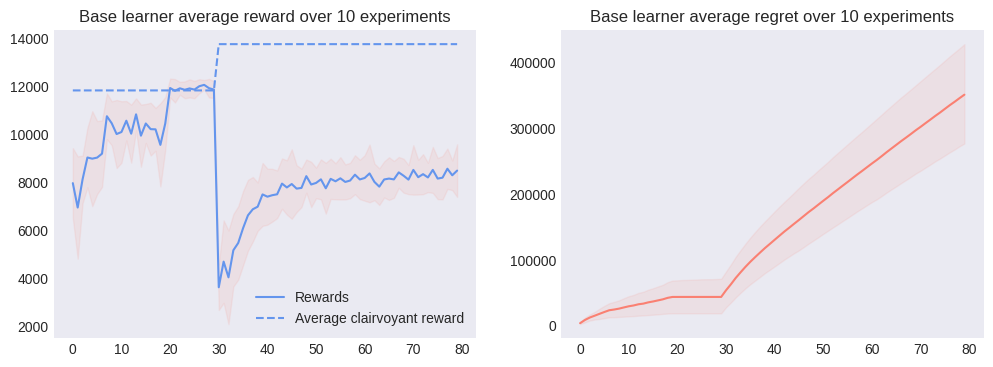
\includegraphics[width=\paperwidth]{img/Graphs/non_stationary/image1.png}}

\end{frame}

% ----------------------------------------

\begin{frame}
\frametitle{Theoretical guarantees}

In addition, if the \textbf{number of breakpoints} $m$ is small enough with respect to the \textbf{time horizon} $T$ to the power of $\alpha$ we have that the \textbf{regret} is of the order $O\left( \vert A \vert T^{\frac{1+\alpha}{2}} \right)$

\end{frame}

% ----------------------------------------
